\lecture{5}{Thu 12 Mar 2020 16:17}{Disturbi della percezione}{

La percezione ha diversi aspetti:
\begin{itemize}
	\item Ricettivo
	\item Costruttivo
	\item Integrativo
\end{itemize}

Non è scindibile dal resto dell'attività psichica (attenzione, coscienza, memoria ed affettività).
Alcuni fenomeni psichici si distinguono tra percettivi e rappresentativi.
\medskip\\
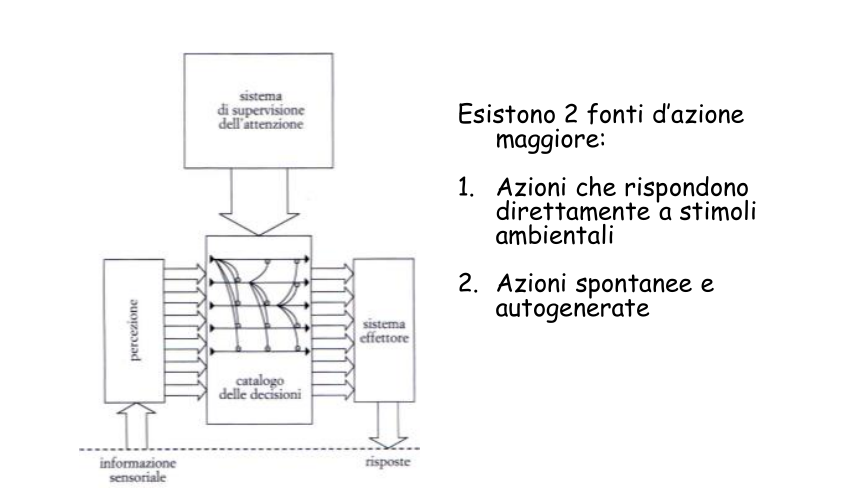
\includegraphics[width=\linewidth]{./images/image5}
\medskip\\

\paragraph{Disturbi della percezione}
Sono considerati sempre disturbi secondari, e si dividono in:
\begin{itemize}
	\item Distorsioni sensoriali, \emph{l'oggetto reale è presente ma viene percepito in modo distorto} 
	\item False percezioni, \emph{illusioni, per esempio gestaltiche} 
\end{itemize}

Le distorsioni sensoriali possono coinvolgere:
\begin{itemize}
	\item Intensità e qualità della percezione 
	\item Componenti emotive della percezione
	\item Dissociazione delle percezioni
\end{itemize}
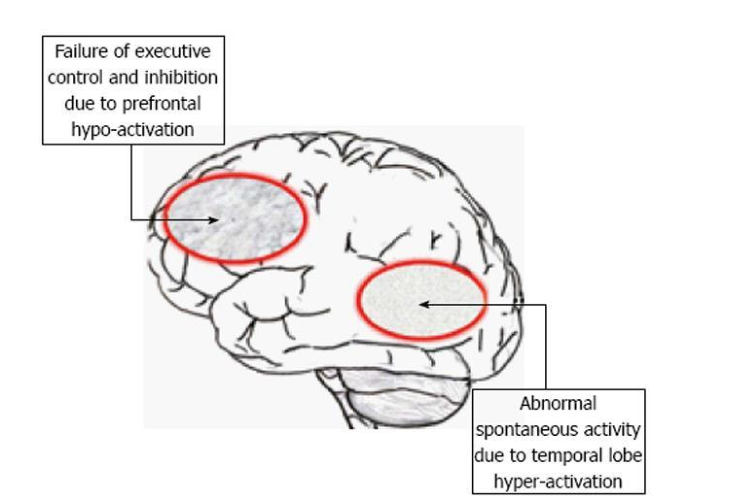
\includegraphics[width=\linewidth]{./images/image6}
\medskip\\
Possiamo chiamare le \textbf{alterazioni dell'intensità} ipo/iperestesie, e intendiamo l'aumentata intensità delle sensazioni, risultato o di intense emozioni o di una riduzione di una soglia fisiologica. L'iperestesia si chiama iperacusia nel caso dell'apparato acustico, e può essere provocata da hangover e ansia, ecc\ldots, mentre l'ipoestesia si dice ipoacusia, e può essere provocata da ADHD, delirium o depressione.

Nel caso del sistema visivo, l'iperestesia può presente in pazienti ipo/maniacali, in caso di aura epilettica o per uso di sostanze, ma anche per esperienze mistiche o innamoramento. L'ipoestesia si può esprimere in ridotta intensità cromatica più comunemente in caso di depressione, che trascina verso il basso ogni altra facoltà mentale.

Le \textbf{alterazioni del senso di familiarità} possono riguardare:
\begin{itemize}
	\item senso di familiarità, come nei deja voe. 
	\item coinvolgimento e vicinanza emotiva
	\item piacevolezza
	\item senso di realtà
\end{itemize}
e si trovano in:
\begin{itemize}
	\item stati di derealizzazione (non patologici, possono essere collegati ad uso di sostanze, o come parte di un attacco di panico per esempio)
	\item disturbi dell'umore (le sensazioni sono percepite 'come se...')
	\item schizofrenia (le sensazioni sono percepite reali)
\end{itemize}

\paragraph{Dissociazione delle percezioni} incapacità di fondere in un unico percetto sensazioni simultanee provenienti dallo stesso oggetto, proveniente in schizofrenia o stati di intossicazione.

Le false percezioni:
\paragraph{Illusione percettiva}consiste nella distorsione di un oggetto esterno reale. Ci sono 3 tipi:
\begin{itemize}
	\item Da completamento (Gestalt)
	\item Emotive (a genesi affettiva) l'agente determinante è lo stato emotivo e sono vanificate dall'attenzione
	\item Pareidoliche (quelle nelle nuvole e nel test di Rorschach)
\end{itemize}
\paragraph{Pseudoallucinazione}  forma intensificata di una rappresentazione, ma sempre interna e senza caratteri deliranti
\paragraph{Allucinazione} percezione senza oggetto e proiettata all'esterno. Non correggibile. L'allucinazione ha tutte le caratteristiche della percezione, si sovrappone perfettamente alla realtà. Possono anche riguardare la percezione interna. Hanno la stessa forza e impatto delle percezioni reali.
\medskip\\
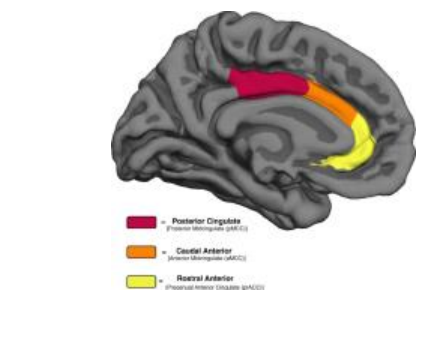
\includegraphics[width=\linewidth]{./images/image7}
\medskip\\
L'unico aspetto che differisce tra percezione normale e allucinazione è il carattere di \textbf{non-privatezza}, ovvero chi allucina non sempre assume che gli altri possano condividere la sua esperienza.
Un ulteriore aspetto delle allucinazioni è l'\textbf{auto-centrismo}. Questo aspetto caratterizza anche i deliri. Sono inoltre pervasive dal punto di vista comportamentale e spesso hanno un forte vissuto emozionale.




















